\documentclass{article}
\usepackage[utf8]{inputenc}
\usepackage{amsmath}
\usepackage{float}
\usepackage{array}
\usepackage{hyperref}
\usepackage{listings}
\usepackage{geometry}
\usepackage{graphicx}
\usepackage[spanish]{babel}


\title{ \textbf{Proyecto Final} }
\author{Martínez Ostoa Néstor Iván \\ \#315618648 \\ Arquitectura Cliente Servidor - 2946} 
\date{Agosto 2021}

\begin{document}

\maketitle


% --------------------------------------------------------------------
% --------------------------------------------------------------------
% --------------------------------------------------------------------
\section{Objetivos}

Realizar una arquitectura cliente servidor en lenguaje C para simular un manejador de base de datos. El proyecto deberá cumplir con lo siguiente: 

\begin{itemize}
    \item El cliente debe enviar un comando al servidor
    \item El servidor debe recibir las instrucciones del cliente y realizar las operaciones correspondientes
    \item El servidor deberá responderle de vuelta al cliente
	\item El servidor deberá ejecutar sus acciones sobre archivos
\end{itemize}


% --------------------------------------------------------------------
% --------------------------------------------------------------------
% --------------------------------------------------------------------
\section{Descripción de la arquitectura}

Como se mencionó en los objetivos, la idea de esta arquitectura será simular un manejador de base de datos en donde el cliente será responsable de ejecutar secuencias de SQL y el servidor de responder a dichas secuencias y manejar los archivos correspondientes de la base de datos. A continuación se especifican las responsabilidades de cada entidad. 

\subsection{Servidor}

Los comandos que el servidor reciba se ejecutarán sobre archivos y éste deberá ser capaz de procesar de manera correcta comandos como el siguiente: \\

\verb|INSERT numcta apellido_paterno apellido_materno nombre(s)| \\ 

donde \verb|numcta| es el número de cuenta del alumno a insertar en la base de datos. El servidor deberá manejar las inserciones mediante archivos cuyo nombre será el valor de \verb|numcta|. Se tendrá que tener un archivo por alumno. Una vez que se realicé la inserción, el servidor deberá responder al cliente con un mensaje de éxito o error en caso de existir uno. 


\begin{figure}[H]
    \centering
    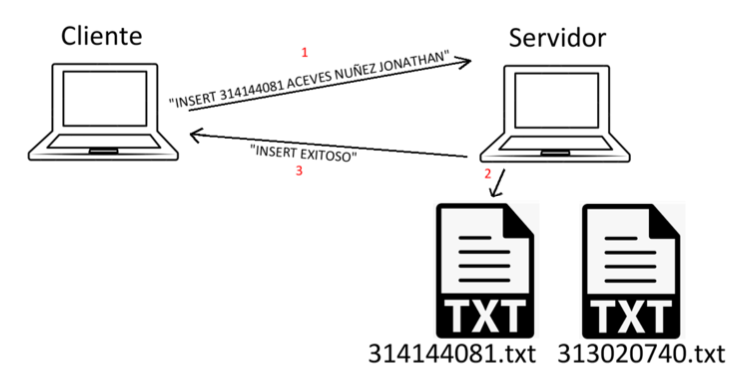
\includegraphics[scale=0.3]{imgs/insert_numcta.png}
    \caption{Ejemplo de inserción de elementos en la base de datos}
    \label{fig:insert_numcta}
\end{figure}

\subsection{Cliente}

Por otro lado, el cliente a parte de poder insertar elementos a la base de datos, será capaz de hacer selecciones con base en un número de cuenta. El cliente, por medio del comando \verb|select numcta| podrá obtener el contenido del archivo \verb|numcta|. Cuando el servidor reciba esta instrucción, deberá responder con el contenido del archivo en caso de que exista. De lo contrario, deberá mandar un mensaje de error. 

\begin{figure}[H]
    \centering
    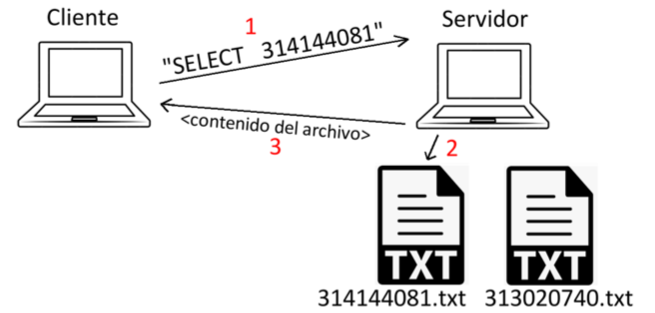
\includegraphics[scale=0.32]{imgs/select_numcta.png}
    \caption{Ejemplo de selección de elementos dentro la base de datos}
    \label{fig:select_numcta}
\end{figure}


% --------------------------------------------------------------------
% --------------------------------------------------------------------
% --------------------------------------------------------------------
\section{Desarrollo}




% --------------------------------------------------------------------
% --------------------------------------------------------------------
% --------------------------------------------------------------------
\section{Conclusiones}




% --------------------------------------------------------------------
% --------------------------------------------------------------------
% --------------------------------------------------------------------
\begin{thebibliography}{}

\bibitem{zamitiz} Zamitiz C. Apuntes de la materia Arquitectura Cliente Servidor. 2021. Facultad de Ingeniería. UNAM

\end{thebibliography}


\end{document}










